\section{Details on data simulation} \label{app:simul}
In the following paragraphs we provide detailed information on the data simulation of a closed population of a hypothetical animal. We used an individual-based model, containing both males and females. We started with a population of 200 1-year old individuals, and fifty time steps were simulated. In this simulated population, body size was a fitness related trait, shaped by an individual's genotype, maternal effects, the environment and its ontogenetic growth. Every year, first food is distributed among all individuals. Subsequently, each individual either survives or dies. Surviving individuals age, grow and then they potentially reproduce. Details on these processes are given below.

\subsection{Simulation of the genotypes} \label{app:simul:gen}
Each diploid individual had a genotype for body size consisting of $10$ independent genes, for each of which there are $10$ alleles (leading to a total of $(10+\frac{10\cdot9}{2})^{10}$ possible genotypes -- i.e. per gene there are 10 ways of being homozygote and $\frac{10\cdot 9}{2}$ way of being heterozygote). The importance of each gene, that is the variance in the additive effects of its alleles, was drawn from a folded normal distribution. Subsequently, the effect of the $10$ homozygotes for this gene was determined by drawing a number from a normal distribution with a standard deviation equal to the importance of that gene. Finally, the genotypic effects of heterozygotes was determined for all pairs of alleles per gene, by drawing a dominance value from a uniform distribution bounded by the additive effects of the two alleles. Based on these values, and assuming no epistasis, we obtained body size genotypic values for all possible genotypes ($10$ homozygotes plus $\frac{10\cdot 9}{2}$ heterozygotes) by summing the additive effects across alleles and genes.

For the first cohort of 200 individuals, individual genotypes were drawn randomly from all possible genotypes, while for subsequent cohorts the genotype was inherited from the parents in a Mendelian way.

\subsection{Birth size} \label{app:simul:birth}
Birth size of individual $i$ ($z^i_0$) was determined as an intercept value $\beta_{z0}$, equal to 10 in our simulation, plus the sum of three processes: genotypic effects, maternal effects and stochasticity.  An individual's genotypic value $b_i$ was determined by the inherited genotype. Second, a fraction $M$ of the size of the mother at the moment of reproduction ($z^i_m$), represented a maternal effect. This maternal effect thus depends on the phenotype of the mother, which in turn is partially determined by her genotype. This fraction $M$ equalled 0.1 in our application. This yielded the expected birth size in absence of stochasticity:

\begin{align}
\zeta_i = \beta_{z0} + b_i + M \cdot z^i_m \text{ .}
\end{align}

Third, we included a random plasticity component, reflecting the experienced micro-environment, drawn from a normal distribution with standard deviation $\sigma_{z0}$, which equalled 0.5 or 1 depending on the scenario (Appendix \ref{app:scenarios}), to obtain an individual's birth weight $z^i_0$.

\begin{align}
z^i_0 = \mathcal{N}(\zeta_i,\sigma_{z0})
\end{align}

\subsection{Growth} \label{app:simul:growth}
Body size increased over time due to growth, which was proportional to body size. There was no heritable variation in growth rate. For one-year-old individuals ($\alpha=1$), mean proportional growth was $\mu_{growth}$, and equalled 1.245. Proportional growth for individual $i$ decreased with age ($\alpha_i$), approaching $1$. 

\begin{align}
\label{eq:meanG}
\gamma_i = (\mu_{growth} +\alpha_i -1) / \alpha_i
\end{align}

Age-dependent proportional growth was further influenced by individual food intake $E_i$, whereby low food availability decreased proportional growth:

\begin{align}
\label{eq:g}
g_i = 1 + (\gamma_i-1) \cdot (\frac{2}{1+e^{-c \cdot E_i}} - 1) \text{ .}
\end{align}

Here, $E_i$ is food availability obtained by individual $i$, and $c$ is a food to growth conversion, which we set at 0.05. To include random plasticity in growth, the yearly realized proportional growth was drawn from a normal distribution, with mean $g_i$ and a standard deviation $\sigma^i_{growth}$, the latter depending on $\gamma_i$, and calculated as

\begin{align}
\label{eq:sigmagrowth}
\sigma^i_{growth} = (\gamma_i-1)/2
\end{align}

To obtain the new body size $z^\prime_i$, proportional growth was multiplied with current body size $z_i$:

\begin{align}
z^\prime_i = \mathcal{N}(g_i,\sigma^i_{growth}) \cdot z_i \text{ .}
\end{align}

Equation \ref{eq:sigmagrowth} implies that variance in growth decreased with age and that individuals could shrink. This led to individual variation in growth within and between years. Individual proportional growth ($g_i$) was not correlated across years. However, because growth was proportional, individuals that grew more in one year, on average also gained more (absolute) size in the next year. 

\subsection{Reproduction} \label{app:simul:repr}
We explicitly modelled variation in the reproductive success of females, but males were randomly assigned to females once the reproductive success of the females was determined. Annual reproductive success of female $i$ ($F_i$) was the product of the reproduction probability $p^i_{repr}$, and the litter size $L_i$.

The probability of reproduction increased with age:

\begin{align}
p^i_{repr} = 1 / (1+\mathrm{exp}(-\alpha_i - \alpha_m)) \text{,}
\end{align}

where $\alpha_i$ is individual age and $\alpha_m$ is the age at which individuals become mature, which is set to 1 in our simulations. This implies that individuals started reproducing one year after their birth with 50\% probability. 
Whether the female $i$ reproduces or not was simply drawn from a Bernouilli distribution:
\begin{align}
\pi_i = \mathcal{B}(p^i_{repr}) \text{ .}
\end{align}

Expected litter size was a function of body size and food availability:

\begin{align}
L_i = \mathrm{exp}(\mathrm{log}(L_{0}) + \beta_{L1} \cdot (z_i-z_0) + \beta_{L2} \cdot (E_i^{1/3}) / 10) \text{ , }
\end{align}

where $L_{0}$ is a baseline reproductive success and was set at 0.5, $\beta_{L1}$ is the strength of the body size effect (set at 0 or 0.04, depending on the scenario; Appendix \ref{app:scenarios}), $\beta_{L2}$ is the effect of food availability (set at 0.1), $E_i$ is the current food availability and $z_0$ is a centering parameter and was set at 15 (approximately the mean mass in the simulated population).
The realized litter size was then drawn from a Poisson distribution and a value of $1$ was added to make sure the litter contains at least one offspring:
\begin{align}
\rho_i = \mathcal{P}(L_i) + 1 \text{ .}
\end{align}
\begin{figure}[ht]
\centering
	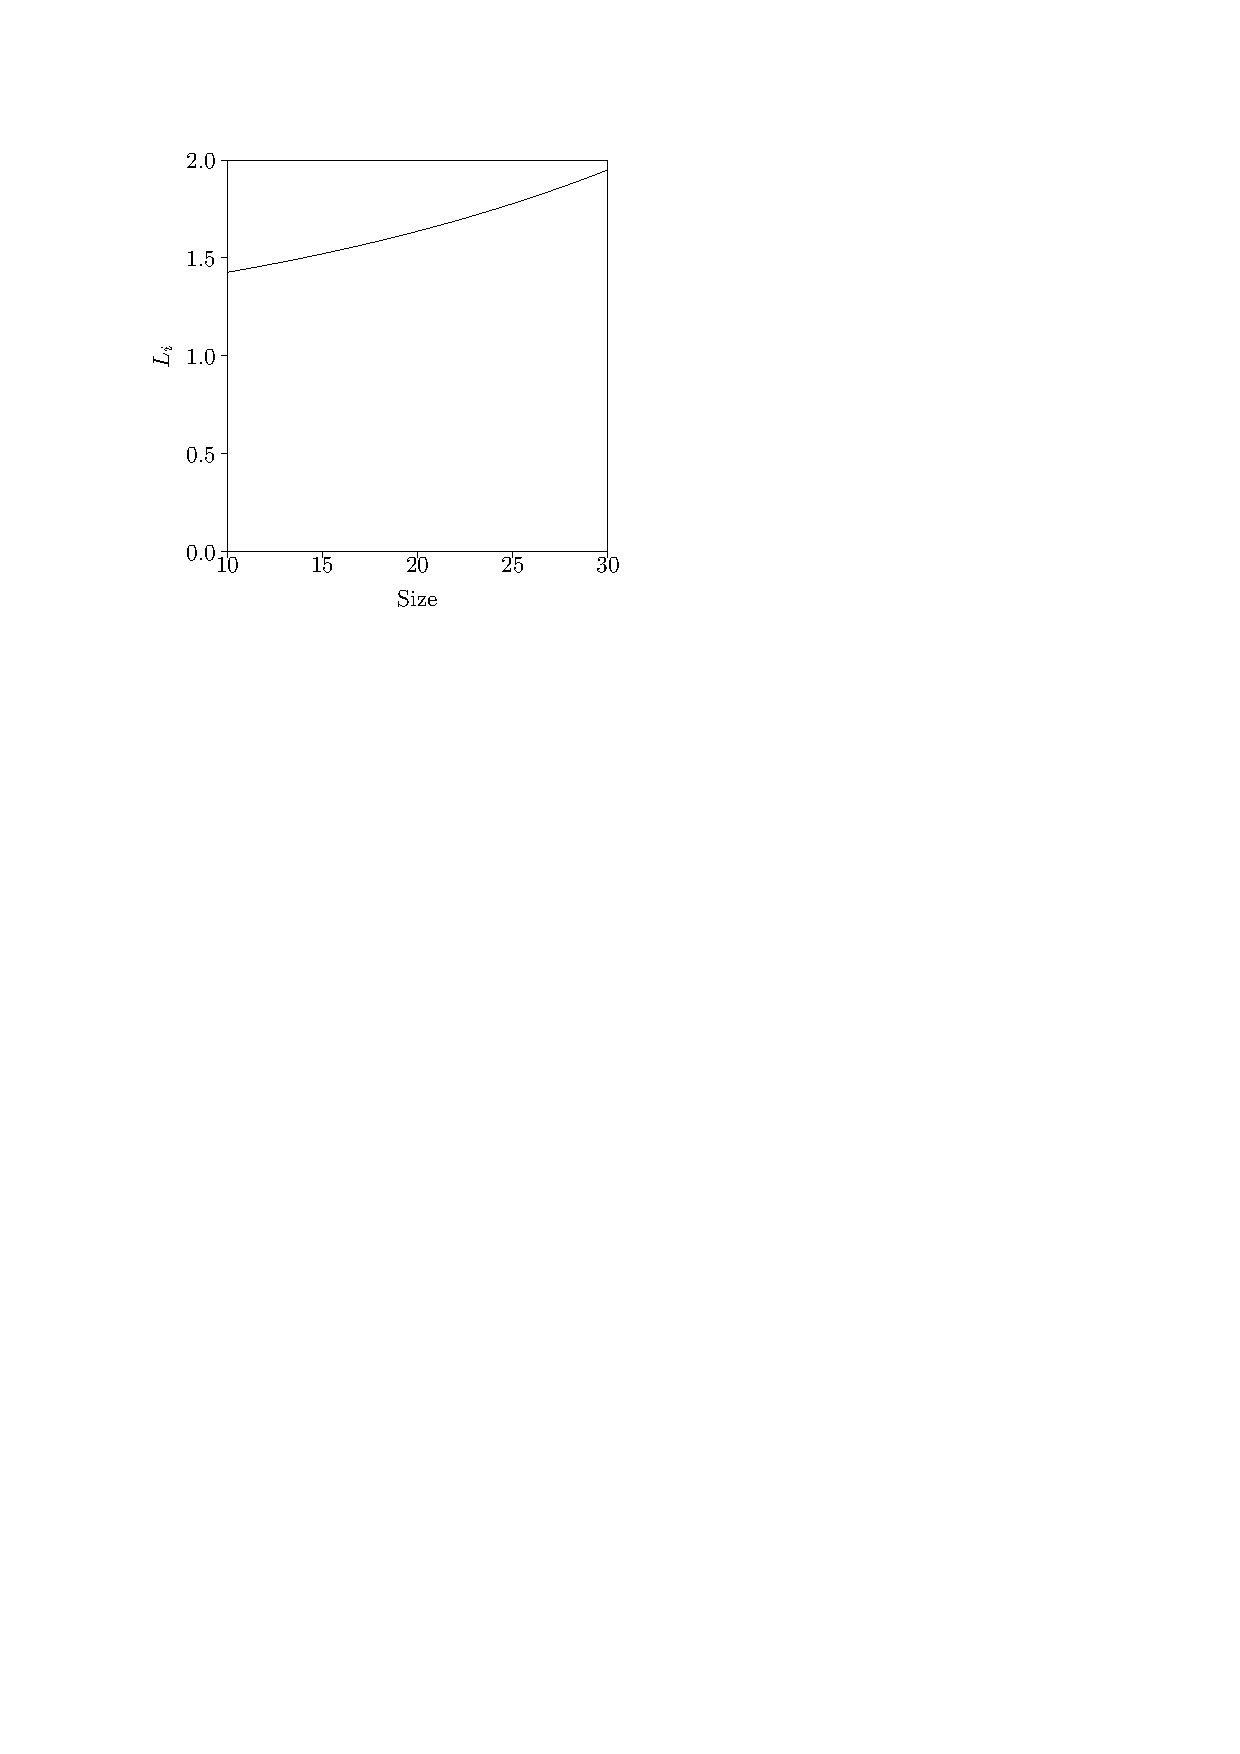
\includegraphics[width=0.5\textwidth]{Appendices/FigS1}
  \caption{\footnotesize Expected reproductive outcome per year as a function of size.}
   \label{SizeRho}
\end{figure}

Individual annual reproductive success was subsequently calculated as
\begin{align}
F_i = \pi_i \cdot \rho_i \text{ .}
\end{align}

\subsection{Survival} \label{app:simul:surv}
Survival was positively affected by food availability and was a function of age, the latter through a bathtub function: survival first increased with age ($\alpha$) but started decreasing after an age of 5, reflecting senescence.
Thus, considering only the effect of age, the survival probability of individual $i$ can be written as
\begin{align}
\phi_{\alpha,i} = 1 - m \cdot \mathrm{exp}(-(\alpha_i-\alpha_s)/4) + \mathrm{exp}((\alpha_i-\alpha_s)\mathrm{log}(2)/(\alpha_m-\alpha_s)) \text{,}
\end{align}
where $m$ is the baseline mortality (0.1), $\alpha_i$ is the current age of $i$, $\alpha_m$ is the maximal age (30) and $\alpha_s$ is the age after which survival decreases again due to senescence (set at 5).
\begin{figure}[ht]
\centering
	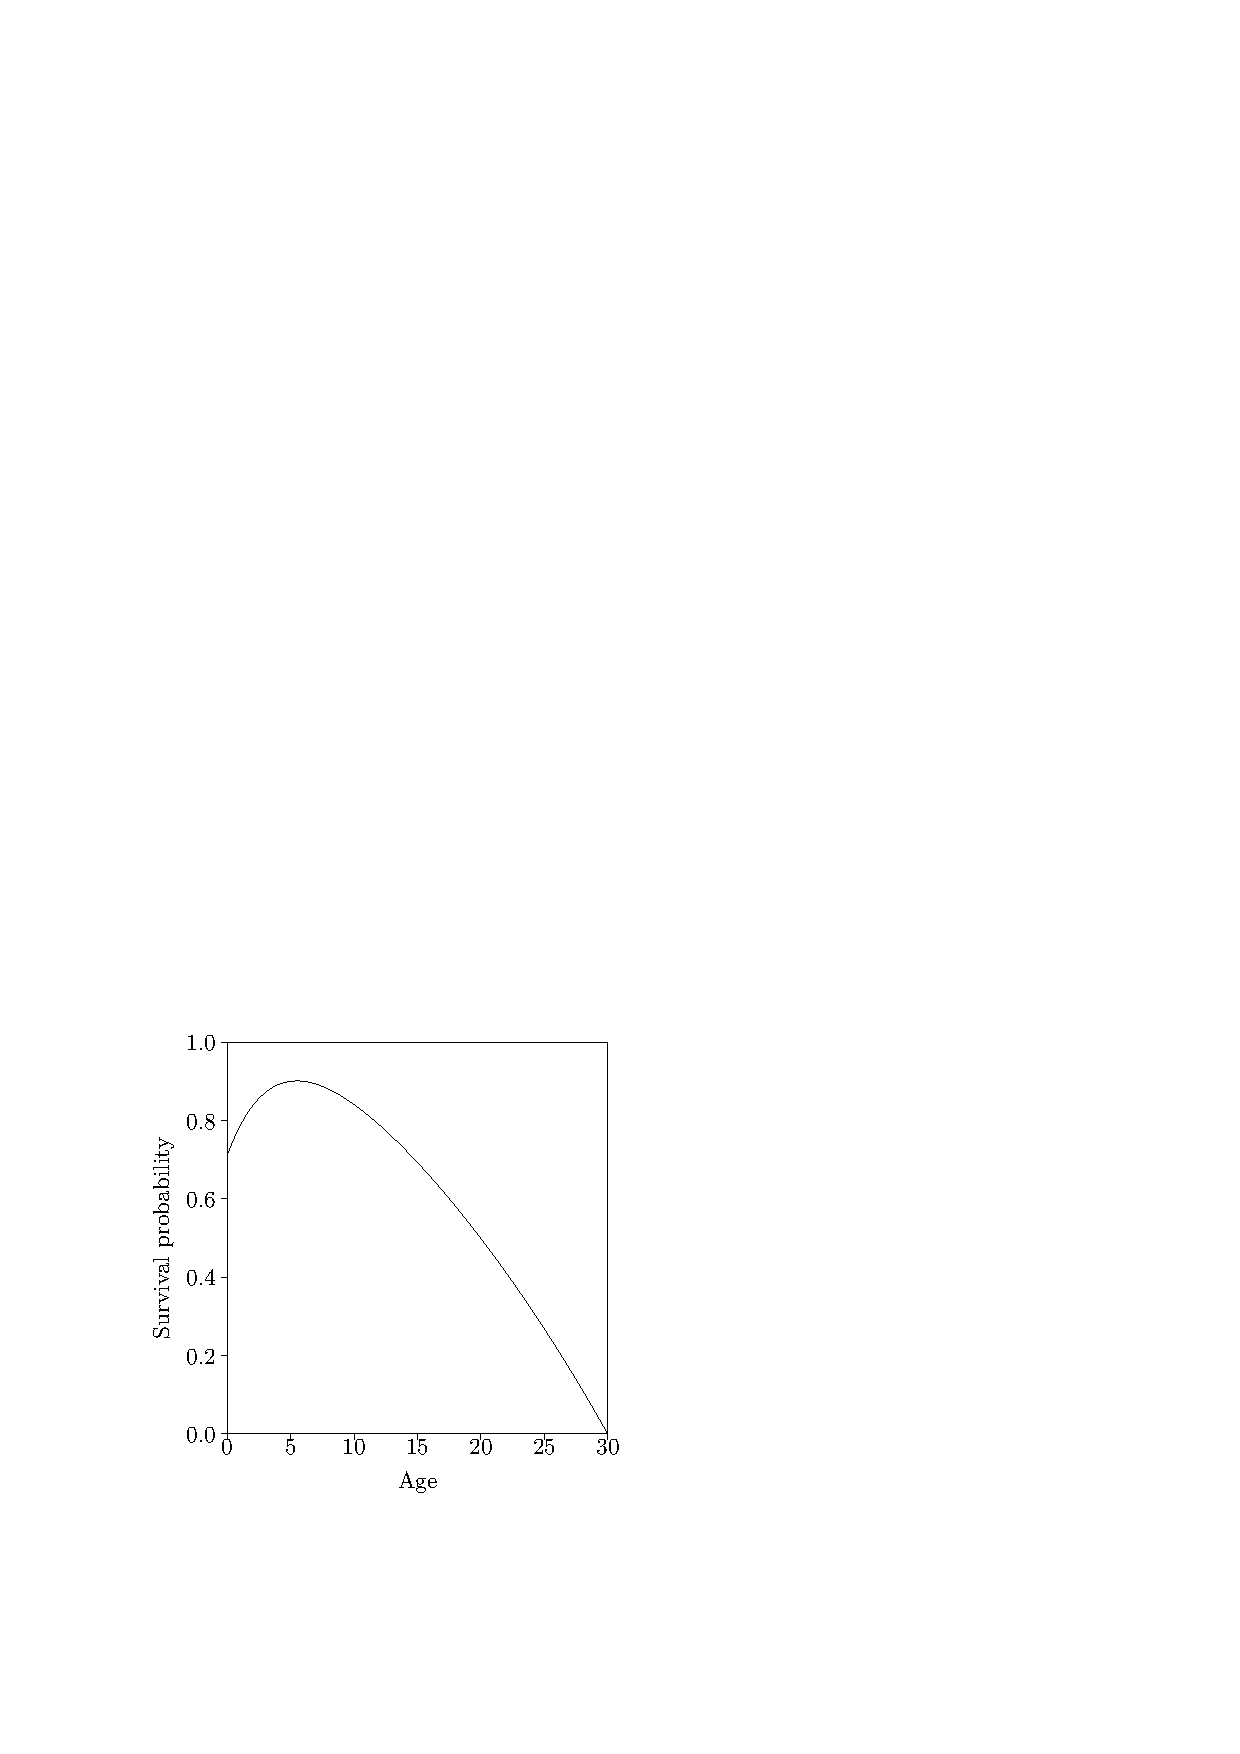
\includegraphics[width=0.5\textwidth]{Appendices/FigS2}
  \caption{\footnotesize Probability of survival to the next year, as a function of age.}
   \label{bathtub}
\end{figure}
Survival also varied depending on the size of the individual ($z_i$) and on the reproductive success during the previous year ($F_i$). Thus, we have:
\begin{align}
\phi_{m,i} = \mathrm{logit}^{-1}(\mathrm{logit}(\phi_0) - \beta_{\phi}(z_i-15)   + F_i h_F) \text{,}
\end{align}
where $\phi_0$ is a baseline survival probability (0.75 in our application), $\beta_{\phi}$ is the linear selection gradient, which was set at either 0 or 0.2 (SI Appendix \ref{app:scenarios}). $h_F$ is the strength of the trade-off between survival and reproduction and was set at 0.01. The survival probability of the individual $i$ is the product of the age-specific survival probability and of the size- and reproduction-specific survival probability:
\begin{align}
\phi_{i} = \phi_{m,i}\phi_{\alpha,i}\text{.}
\end{align}
%\begin{figure}[ht]
%	\includegraphics[width=0.5\textwidth]{Appendices/SizePhi}

%  \caption{Probability of survival to the next year, as a function of size.}
%   \label{survivalsize}
%\end{figure}

Finally, a shortage of food acquisition by the individual ($E$) can decrease survival. If $E<40$:
\begin{align}
	\phi_i^{\prime}= 1 - (1-\phi_{i})(E/40)^{1/2}\text{.}
\end{align}

\subsection{Food availability} \label{app:simul:food}
Total food availability differed per year and the amount an individual obtained influenced individual growth and reproduction. The expected total amount of food available in year $t$ started to decrease after year 10, and can be written as

\begin{align}
   E_{\mu} (t) = 
\begin{cases}
    \mu_E, & \text{if } t \leq 10 \text{ ,}\\
    \mu_E + (t-10) \cdot \beta_E \text{ ,}             & \text{ otherwise.}
\end{cases}
\end{align}

We set $\mu_E$ at 15000 and $\beta_E$ is the yearly rate of decrease after year 10, and was set at -200.

To include random variation in food availability, the realized amount of food available was drawn from a folded normal distribution, whereby the variance of the Gaussian ($\mathcal{N}$) was proportional to the mean.

\begin{align}
E_{tot} (t) = \lvert \mathcal{N}(E_{\mu}(t),\sigma_E)\rvert
\end{align}

In our simulations, $\sigma_E$ was set at $E^t_{\mu}/10$. The total amount of food was divided over all $N$ alive individuals, whereby some individuals obtained more than others. The amount of food that an individual obtained was assigned randomly. To do so, each year ($t$), a measure of successful foraging ($\eta_i^t$) was assigned to each individual. For each individual, this was a number between $0.3$ and $1$ from a uniform distribution, i.e.:
\begin{align}
\eta_i (t) = \mathcal{U}(0.3,1) \text{ , }
\end{align}

Using these, we calculated the food amount obtained by individual $i$ at time $t$ as

\begin{align}
E_i (t) = \frac{E_{tot} (t) \cdot \eta_i (t)}{ \sum_{i=1}^{N} \eta_i (t)} \text{ . }
\end{align}

\clearpage
\subsection{Scenarios} \label{app:scenarios}
We have simulated data under four biologically different scenarios. These scenarios are presented below. For each scenario, we have ran 100 replicates, resulting in a total of 400 datasets.
\begin{table}[ht]
\centering
\caption{Simulated scenarios} 
\label{coeff}
\begin{tabularx}{\textwidth}{lXX}
  \hline
Scenario & Description & Parameter value \\ 
  \hline
$s_0h_-$ & Low genetic variance \newline High plasticity in birth size \newline No fertility selection \newline No viability selection & $V_A \approx 1$ \newline $\sigma_{z_0}=1$ \newline $\beta_{L1}=0$ \newline $\beta_{\phi}=0$  \\ \hline
$s_0h_+$ & High genetic variance \newline Low plasticity in birth size \newline No fertility selection \newline No viability selection& $V_A \approx 5$  \newline $\sigma_{z_0}=0.5$ \newline $\beta_{L1}=0$ \newline $\beta_{\phi}=0$ \\ \hline
$s_+h_-$ & Low genetic variance \newline High plasticity in birth size \newline High fertility selection \newline High viability selection& $V_A \approx 1$ \newline $\sigma_{z_0}=1$ \newline $\beta_{L1}=0.04$ \newline $\beta_{\phi}=0.2$ \\ \hline
$s_+h_+$ & High genetic variance \newline Low plasticity in birth size \newline High fertility selection \newline High viability selection& $V_A \approx 5$  \newline $\sigma_{z_0}=0.5$ \newline $\beta_{L1}=0.04$ \newline $\beta_{\phi}=0.2$ \\ 
  \hline
\end{tabularx}
\end{table}

\subsection{Full R code}
The R code that was used to generate the analysed datasets is provided as additional supplementary information on \href{https://github.com/koenvanbenthem/Disentangling_Dynamics_IBM}{GitHub} (doi: \href{https://doi.org/10.5281/zenodo.59412}{10.5281/zenodo.59412}).